\documentclass[10pt,xcolor={table,dvipsnames},t]{beamer}
\usetheme{UCBerkeley}
\usepackage{ctex}

\title{Streo PIV principle}
\subtitle{Part I: Stereo PIV in perspective of pinhole camera model}
\author{刘宁}
\institute{浙江大学}
\date{\today}

\begin{document}

\begin{frame}
  \titlepage
\end{frame}

\section{Introduction}

\begin{frame}{One big picture: Stereo PIV principle}
  一些废话定义:
  \begin{itemize}
    \item Stereo PIV 是一种基于双目立体视觉原理的三维流场测量方法。
    \item 其核心是通过两台相机对同一平面上的粒子进行拍摄,利用视差原理重建三维流场。
  \end{itemize}
  
  \begin{figure}
    \centering
    \includegraphics[width=0.65\textwidth]{figures/spiv-big-picture.png}
    \caption{Stereo PIV原理示意图。}
  \end{figure}
\end{frame}

\begin{frame}{Camera: a 3D world to 2D image mapping function}
    \begin{align*}
      \mathbf{x} = P\mathbf{X}.
    \end{align*}

      \begin{figure}
        \centering
        \includegraphics[width=0.8\textwidth]{figures/pinhole-camera-model.png}
        \caption{Pinhole camera model. \href{https://www.cs.cmu.edu/~16385/s17/Slides/11.1\_Camera\_matrix.pdf}{Source}}
      \end{figure}
\end{frame}

\begin{frame}{One big picture: Stereo PIV principle}
Stereo PIV 不仅需要 $XY$ 平面的映射关系
\footnote{此处预设了 object plane 厚度为 $0$,且与 $Z=0$ 平面重合,因此映射函数不显含 $Z$,其实此处的单台相机映射函数为;
$$
\begin{cases}
x = F(X, Y, 0),  \\
y = G(X, Y, 0).
\end{cases}
$$
考虑到实际激光平面厚度为 $1\sim 2 \mathrm{mm}$,相机景深也不为 $0$,上述映射函数缺乏 $Z$ 方向信息。}
,而且需要知道映射函数的 $z$ 向导数

\footnote{stereo calibration相当于估计映射函数的马克劳林一阶余项,在标定时控制 $(X,Y)$ 不变,在激光面范围内仅沿 $Z$ 方向移动标定板 $dZ$,通过不同相机上的位移 $(dx, dy)$ 变化近似得到 $\frac{ \partial F }{ \partial Z }$ 和 $\frac{ \partial G }{ \partial Z }$ 
$$
\begin{cases}
dx = \frac{ \partial F }{ \partial Z }|_{(X,Y,0)}\cdot dZ, \\
dy = \frac{ \partial G }{ \partial Z } |_{(X,Y,0)}\cdot dZ.
\end{cases}
$$}
,用以后续重建三维流场。

基于上述物理信息,在Stereo PIV中的左右相机重构三维流场可以变换为求解超定线性方程组的问题(最暴力但缺乏物理依据的解法SVD)
\end{frame}


\begin{frame}{One big picture: Stereo PIV principle}
Stereo PIV 不仅需要 $xy$ 平面的映射关系,而且需要知道映射函数的 $z$ 向导数 ,用以后续重建三维流场。

基于上述物理信息,在Stereo PIV中的左右相机重构三维流场可以变换为求解超定线性方程组的问题(SVD!)

$$
\begin{bmatrix}
dx_{left} \\
dy_{left} \\
dx_{right} \\
dy_{right}
\end{bmatrix}
= 
\begin{bmatrix}
\displaystyle\ \frac{ \partial F_{left} }{ \partial X } & \displaystyle\ \frac{ \partial F_{left} }{ \partial Y } & \displaystyle\ \frac{ \partial F_{left} }{ \partial Z }  \\
\displaystyle\ \frac{ \partial G_{left} }{ \partial X } & \displaystyle\ \frac{ \partial G_{left} }{ \partial Y } & \displaystyle\ \frac{ \partial G_{left} }{ \partial Z }  \\
\displaystyle\ \frac{ \partial F_{right} }{ \partial X } & \displaystyle\ \frac{ \partial F_{right} }{ \partial Y } & \displaystyle\ \frac{ \partial F_{right} }{ \partial Z }  \\
\displaystyle\ \frac{ \partial G_{right} }{ \partial X } & \displaystyle\ \frac{ \partial G_{right} }{ \partial Y } & \displaystyle\ \frac{ \partial G_{right} }{ \partial Z }
\end{bmatrix}
\begin{bmatrix}
dX \\
dY \\
dZ
\end{bmatrix}.
$$
两边除以$dt$ ,右边项即是三维速度矢量。

\end{frame}

\begin{frame}{Frame vs Coordinate transformation}

  \begin{columns}
    \begin{column}{0.5\textwidth}
\begin{itemize}
  \item Frame transform matrix
  \begin{align*}
    F = \begin{bmatrix}
    \mathbf{R} & \mathbf{t} \\
    \mathbf{0}^T & 1
    \end{bmatrix}.
  \end{align*}
 \item Coordinate transform matrix
   \begin{align*}
    F^{-1} = \begin{bmatrix}
    \mathbf{R}^T & -\mathbf{R^T t} \\
    \mathbf{0}^T & 1
    \end{bmatrix}.
   \end{align*}
\end{itemize}
    \end{column}

    \begin{column}{0.5\textwidth}
      \begin{figure}
        \centering
        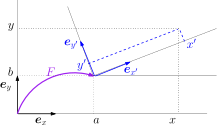
\includegraphics[width=0.8\textwidth]{figures/coord-frame.pdf}
        \caption{Frame vs Coordinate transformation. \href{https://staff.fnwi.uva.nl/r.vandenboomgaard/ComputerVision/LectureNotes/MATH/homogenous.html\#coordinate-frame-transforms}{Source}}
      \end{figure}
    \end{column}
  \end{columns}

\end{frame}

\begin{frame}{Extrinsic parameters: camera pose}
  \begin{columns}
    \begin{column}{0.3\textwidth}
      \begin{itemize}
        \item 相机外参描述相机在世界坐标系中的位置和方向。
        \item 通常用旋转矩阵 $\mathbf{R}$ 和平移向量 $\mathbf{t}$ 表示。
      \end{itemize}
    \end{column}

    \begin{column}{0.7\textwidth}
      \begin{figure}
        \centering
        \includegraphics[width=0.9\textwidth]{figures/extrinsic-parameters.png}
        \caption{Extrinsic parameters of a camera. \href{https://www.cs.cmu.edu/~16385/s17/Slides/11.1\_Camera\_matrix.pdf}{Source}}
      \end{figure}
    \end{column}
  \end{columns}
  
\end{frame}

\end{document}
